
\section{Neural Feature Extractors}
\label{sec:nn-features}

The Markov Network of Section~\ref{sec:markov-networks} decomposes the
score over nodes and edges. All input-dependent information enters
through the \emph{unary} potentials $f_{v}(x, y_{v})$; the pairwise
term is kept observation-independent (see
Section~\ref{subsec:backbone-interface}). For symbolic inputs
a simple linear or look-up mapping is sufficient, but for visual
inputs --- images of handwritten digits --- a representation must be
learned. This thesis therefore uses a neural network as the unary
feature extractor and trains it jointly with the pairwise
matrix $W$.
Section~\ref{subsec:backbone-interface} fixes an abstract
interface for the backbone so that the actual network used ---
linear or convolutional --- can be plugged in interchangeably.

\subsection{Backbone interface}
\label{subsec:backbone-interface}

Let $g_{\theta} \colon \mathcal{X}_{\mathrm{node}} \to \mathbb{R}^{K}$
denote the neural \emph{backbone} with parameters $\theta$. It is
applied per node: for each $v \in V$, the input assigned to that node
(an image, a one-hot vector, \ldots) is passed through the same
network, and the $K$-dimensional output is taken as the vector of
unary scores,
\begin{equation}
    f_{v}(x, a) \;=\; \bigl[\, g_{\theta}(x_{v}) \,\bigr]_{a},
    \qquad a \in \mathcal{Y}.
    \label{eq:nn-unary}
\end{equation}
Parameters are shared across all positions, so the same network
processes every node independently.

The pairwise potentials are kept observation-independent: $f_{vv'}(a, b) = W_{a, b}$, where $W \in \mathbb{R}^{K \times K}$ is a
learned matrix shared across all edges. The full MN score then reads
\begin{equation}
    f(x, y) \;=\; \sum_{v \in V}
    \bigl[ g_{\theta}(x_{v}) \bigr]_{y_{v}}
    \;+\; \sum_{\{v, v'\} \in E} W_{y_{v},\, y_{v'}},
    \label{eq:nn-mn-score}
\end{equation}
and the trainable parameters are $(\theta, W)$ --- the neural
backbone parameters together with the pairwise matrix.

\subsection{Concrete backbone families}

When the per-cell input $x_v$ is an image of a handwritten digit,
the backbone $g_\theta$ is a neural network mapping the image to
a $K$-dimensional vector of class scores. CNNs in particular
exploit translation invariance and local connectivity through
stacks of convolutional layers with non-linearities and spatial
pooling, followed by a fully connected output head of size $K$,
and are the de-facto choice for MNIST-style digit
recognition~\cite{LeCun1998}. This thesis considers two
concrete backbone families used in the experiments --- a linear
baseline and LeNet-5 --- and additionally supports an extension
point for external backbones. The abstract interface of
Section~\ref{subsec:backbone-interface} accepts either of them
without modification.

\paragraph{Linear baseline.} For symbolic inputs --- where the
per-cell input is the one-hot encoding of the observation digit
--- a single linear layer maps the $K$-dimensional one-hot vector
to $K$ logits. This serves as a sanity-check lower bound on what
the M\textsuperscript{3}N decision layer can extract from a
minimal unary feature extractor.

\paragraph{LeNet-5.} The classical CNN family introduced by LeCun
et al.~\cite{LeCun1998} for handwritten-digit recognition. This
thesis uses the modern variant of LeNet-5 popularised in
\emph{Dive into Deep Learning}~\cite{d2l-lenet}: three
convolutional blocks --- the first two each followed by max
pooling, the third operating on a $5 \times 5$ feature map and
collapsing it to $1 \times 1$ --- followed by two fully connected
layers (Figure~\ref{fig:lenet5}). Differences from the original
1998 paper are ReLU activations in place of $\tanh$, max-pooling
in place of average pooling, and the collapsed third convolution
in place of an additional fully connected layer. LeNet-5 is the
primary backbone used on visual benchmarks in this thesis, with
the exact layer sequence (channel counts, activation functions,
output dimensionality $K = 9$ on Sudoku and $K = 10$ on visual
HMC) listed in Chapter~\ref{chap:method}.

\begin{figure}[htbp]
\centering
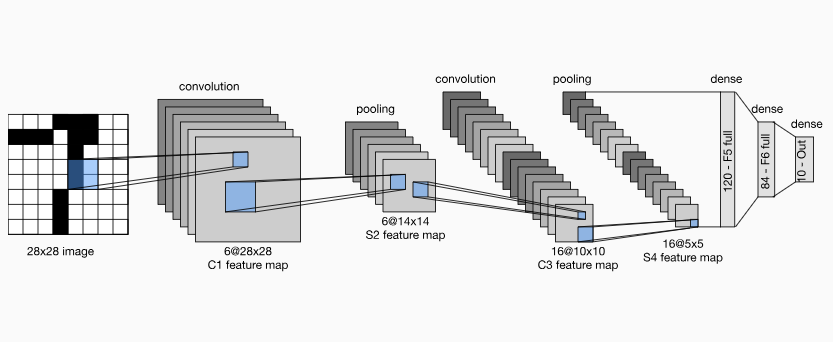
\includegraphics[width=0.9\textwidth]{figures/lenet5}
\caption[LeNet-5 architecture]{LeNet-5 architecture (d2l.ai
variant): three convolutional blocks (the third operating on a
$5 \times 5$ feature map and collapsing it to $1 \times 1$),
followed by two fully connected layers. Image
from~\cite{d2l-lenet}.}
\label{fig:lenet5}
\end{figure}

\paragraph{Wrapped backbones.} The library also accepts any
external network matching the backbone interface, including
modules from \texttt{torchvision} (e.g., ResNet variants) wrapped
with an output head of size $K$. This route is supported in the
implementation but is not exercised in the experiments of this
thesis.

\subsection{End-to-end training}
\label{subsec:end-to-end}

A central design choice is to train $\theta$ and $W$ \emph{jointly}
through a single structured loss: the backbone receives gradients
only through the structured-hinge loss of
Section~\ref{subsec:structured-hinge} (on chains) or the LP-M3N
loss of Section~\ref{subsec:lp-m3n} (on general graphs), never from
a stand-alone per-node classification target. This contrasts with
the two-stage baseline (Chapter~\ref{chap:method}), in which
perception (an OCR classifier) is trained first and its outputs are
only then handed to a hard-coded solver.

Joint training is made possible by the fact that both structured
losses of Section~\ref{sec:learning-mn} are piecewise differentiable
in the unary potentials and, via the chain rule through $g_{\theta}$,
in the backbone parameters. Automatic differentiation in PyTorch
handles the propagation transparently; subgradients of the relevant
$\max$ operations are given by indicators at the arg-max. This style
of neuro-symbolic architecture --- a neural network supplying
evidence to a structured decision layer --- has been explored with
several alternative back-ends, most prominently SATNet, which
replaces the Markov Network with a differentiable MAXSAT
solver~\cite{wang2019satnet}.
